\section{Prozessverwaltung}
Als Prozessverwaltung wird hauptsächlich das Verwalten von Prozessen durch das Betriebssystem verstanden (Vgl. http://www.lowlevel.eu/wiki/Prozessverwaltung). Jeder Prozess besitzt eine eindeutige Identifikation (PID), durch welche dieser vom System angesprochen werden kann. 

\subsection{Prozesszustände}
Jeder Prozess besitzt zu einem bestimmten Zeitpunkt einen fix definierten Zustand, d.h. es können keine Inkonsistenzen auftreten. Abbildung \ref{fig:Process-states} zeigt die verschiedenen Zustände eines Prozesses sowie die jeweilig erlaubten Übergänge zu einem anderen Zustand auf.

\begin{figure}[H]
	
\includegraphics[scale=0.60]{chapters/processmanagement/figures/todo}
	\caption{Erlaubte Prozesszustände und Prozessübergänge}
	\label{fig:Process-states}
\end{figure}

Im folgenden wird eine detaillierte Erklärung zu den einzelnen Zuständen aus Abbildung \ref{fig:Process-states} gegeben.

\begin{description}
	\item[Ready] \hfill \\
	Der Zustand ready tritt ein, wenn ein Prozess bereit wäre um ausgeführt zu werden. 
	
	\item[Running] \hfill \\
	Ein Prozess weist diesen Zustand auf, wenn er gerade ausgeführt wird. Es gibt immer nur einen running Prozess zu einem bestimmten Zeitpunkt.
	
	\item[Blocked] \hfill \\
	XXX
	
	\item[Sleeping] \hfill \\
	XXX	
	
	\item[Free] \hfill \\
	XXX
\end{description}

Es gibt unterschiedliche Zustandsübergänge, welche im Betriebssystem erlaubt sind. Tabelle \ref{table:State-transition} stellt die verschiedenen Übergänge mit einem dazu passenden Beispiel dar.

\begin{table}[H]
\begin{tabular}{p{3cm} | p{3cm} | p{6cm}}
  \textbf{Ausgangszustand} & \textbf{Nächster Zustand} & \textbf{Beispiel} 
  \\ \hline
  Ready & Running & XXX \\
  Running & Blocked & XXX \\
  Running & XXX & XXX \\
  XXX & XXX & XXX \\
  
 \end{tabular}
 \caption{Erlaubte Zustandsübergänge mit Beispiel}
 \label{table:State-transition}
\end{table}

\subsection{Scheduler Eigenschaften}
Der Scheduler weißt eine Zeitscheibe von $10ms$ auf, d.h. jeder Prozess hat $10ms$ bevor er gewechselt wird. Sollte ein anderer Prozess zur Verfügung stehen wird dieser genommen ansonsten bekommt der gleicher Prozesse erneut eine Zeitscheibe von $10ms$. Diese Zeitscheibendauer wurde aufgrund mehrerer Aspekte gewählt: eine zu große Zeitscheibe $>$ $100ms$ würde merkbaren Verzögerungen im Betriebssystem führen, bei einer zu kleinen Zeitscheibe $<$ $1ms$ würde die benötigte Zeit für einen Wechsel im Vergleich zu lange dauern. Durchgeführte Performanztests sind im Kapitel XXX aufgeführt. \\ \\
Das verwendete Schedulingverfahren ist Round Robin. Bei der Verwendung eines Verfahrens mit Prioritäten hätte der Fall mit einem hoch priorisierten Prozesse beachtet werden müssen. Ein Beispiel dazu: Es gibt drei Prioritäten (hoch, mittel und niedrig). Die Konsole wird als hoch eingestuft alle anderen Prozesse sind niedriger priorisiert. Wie bekommt nun ein mittel/niedrig priorisierter Prozess eine Zeitscheibe?

\subsection{Vorgehen bei der Prozessverwaltung}
Das Vorgehen bei der Prozessverwaltung wird im Sequenzdiagramm von Figure \ref{Sequencediagram} dargestellt. Ein Client übergibt dem ProcessManager die Aufgabe einen Prozess zu erzeugen. Dieser delegiert das Erzeugen des Prozesses an den Scheduler weiter. Hierbei ist zu beachten, dass die Metadaten vom Prozess nicht weitergegeben werden. Der Scheduler speichert sich diesen neuen Prozess in seiner Prozesstabelle ab. Das MemoryManagement dient zum Allokieren von benötigtem Speicherplatz für den neuen Prozess. Der erzeugte Prozess wird an den ProcessManager zurückgegeben, wobei dieser noch MetaInformationen beifügt (z.B. den Namen des Prozesses). Dem Client wird am Ende mitgeteilt, ob das Erzeugen erfolgreich war. Ein alternativer Rückgabeparameter wäre die PID, wobei hier darauf zu achten ist, dass im Fehlerfall eine ungültige PID zurückgeliefert wird.

\begin{figure}[H]
	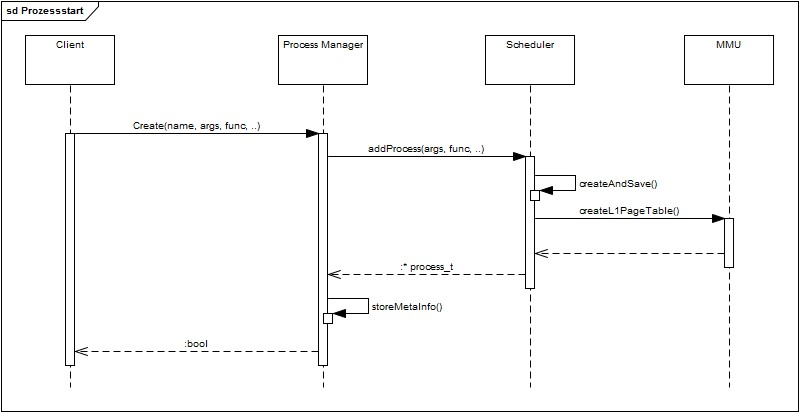
\includegraphics[scale=0.60]{chapters/processmanagement/figures/processmanagement-sequence-diagram}
	\caption{Sequenzdiagramm der Prozessverwaltung}
	\label{fig:Sequencediagram}
\end{figure}

\pagebreak 